%%
%% Streams Plugin
%%  - Generic Wrapper f�r Stream-API
%%  - Abbildung data-items => IOObject, Processor -> Operator,...
%%  - Stream-IOObject => "file handle", lazy reading/evaluation vs. "lade sofort alles in RAM"
%%  - (continuous) Stream-Process => Sub-Process in RapidMiner
%%  - Anbindung/Integration anderer/alter Operatoren
%%
\section{\label{sec:plugin}RapidMiner Streams-Plugin}
The \plugin\ provides RapidMiner operators for the basic building
blocks of the \streams API using a simple wrapper approach to directly
reuse the processor implementations of most of the \streams
packages. 
%Only a very few special processor have been required to be
%re-written so far. 

The operators of the \plugin\ are automatically created from the
processor and data stream implementations using the \textsf{RapidMiner
  Beans} library. This uses reflection and Java annotations to
automatically extract and set parameter types for the wrapping
operators.
Figure \ref{fig:pluginArchitecture} gives an overview over the
\plugin.  The \streams API serves as an abstraction layer providing
implementations of the basic elements identified in Section
\ref{sec:abstraction}.

\begin{figure}[h!]
\begin{center}
\begin{tikzpicture}[scale=0.75]

  \fill[fill=rapidi!60] (-0.5,6.5) -- (-0.5,2.45) -- (12.5,2.45) -- (12.5,6.5);
  \node at (6,5.75) { 
\includegraphics[scale=0.4]{graphics/RapidMinerLogo.jpg} };

  \draw[draw=blue!40,fill=blue!18] (0,1.3) -- (12,1.3) -- (12,2.4) -- (0,2.4) -- (0,1.3);
  \node at (6,1.9) { \textsf{Streams API} };
  
  \draw[draw=blue!50,fill=blue!18] (0,0.2) -- (4,0.2) -- (4,1.2) -- (0,1.2) -- (0,0.2) ;
  \node at (2,0.7) { \textsf{Streams Core} };

  \draw[draw=green!50,fill=green!10] (4.1,0.2) -- (8.1,0.2) -- (8.1,1.2) -- (4.1,1.2) -- (4.1,0.2) ;
  \node at (6,0.7) { \textsf{Streams Mining} };

  \draw[draw=green!40,fill=green!10] (8.2,0.2) -- (8.4,0.2) -- (8.4,1) -- (11.8,1) -- (11.8,0.2) -- (12,0.2) -- (12,1.2) -- (8.2,1.2) -- (8.2,0.2) ;

  
  \draw[draw=black!40,fill=black!10]  (8.5,0) -- (8.5,0.9) -- (11.7,0.9) -- (11.7,0);
  \node at (10.1,0.5) {\textsf{MOA}};


  \draw[draw=blue!40,fill=black!14] (0,2.5) -- (4,2.5) -- (4,3.75) -- (10,3.75) -- (10,5) -- (0,5) -- (0,2.5);
  \node at (5,4.3) { \textsf{Streams Plugin} };

  \draw[draw=rapidiText!80,fill=rapidi!18] (4.1,2.5) -- (12,2.5) -- (12,5) -- (10.1,5) -- (10.1,3.65) -- (4.1,3.65) -- (4.1,2.5);
  \node[color=rapidiText!80] at (9,3.05) { \textsf{RapidMiner Beans} };


\end{tikzpicture}
\end{center}
\caption{\label{fig:pluginArchitecture}The architecture of the
  \textsf{Streams Plugin}, built on top of the \streams API. The
  packages marked as green are work in progress and have not yet been
  fully integrated.}
\end{figure}

\subsection{A Stream Process within RapidMiner}
The elements for {\em streams} and {\em processors} are represented by
RapidMiner operators. The continues {\em process} is mapped to a
RapidMiner subprocess. Figure \ref{fig:rapidMinerStream} shows a
stream process within RapidMiner.

\begin{figure}[h!]
  \begin{center}
    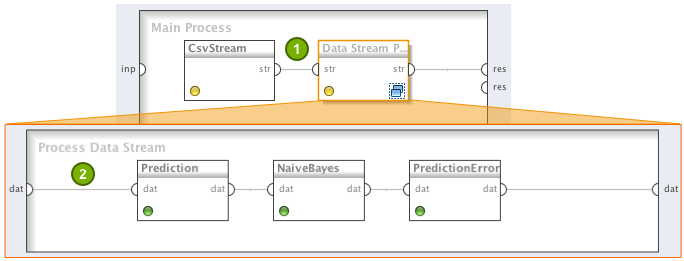
\includegraphics[scale=0.4]{graphics/StreamProcess.png}
  \end{center}
  \caption{\label{fig:rapidMinerStream}A continuous stream process in
    RapidMiner. The top process shows a stream operator and the stream
    process as a subprocess. The edge \pointer{1} represents a data
    stream object. Within the stream subprocess, IOObjects transported
    are single data items (edge \pointer{2}).}
\end{figure}


\subsection{Control Flow and Anytime Services}
Operators that relate to processors implementing a {\ttfamily Service}
interface will be automatically registered as services within a
RapidMiner naming service provided by the \plugin. They can be
referenced by consuming operators using a simple drop-down select box
within the operator parameter view of RapidMiner.

For accessing services or monitoring from outside the continous
streaming process, the \plugin\ integrates an embedded web server that
exports services via a web service interface. Currently services are
exported via this embedded web server using the simple JSON-RPC
protocol \cite{jsonRPC} and a local RMI registry.

%\section{``Power of Abstraction'''}
%
%\section{The RapidMiner Data Stream Plugin}
%\subsection{Architecture}

%\newpage
%
%Documentation with markdown
%
%\begin{figure}
%  \begin{center}
%    \includegraphics[scale=0.4]{doc.png}
%  \end{center}
%\end{figure}